% Created 2023-06-04 Sun 20:15
% Intended LaTeX compiler: lualatex
\documentclass[11pt]{article}
\usepackage{graphicx}
\usepackage{longtable}
\usepackage{wrapfig}
\usepackage{rotating}
\usepackage[normalem]{ulem}
\usepackage{amsmath}
\usepackage{amssymb}
\usepackage{capt-of}
\usepackage{hyperref}
\DeclareExerciseCollection{ListaMisturas}
\DeclareExerciseCollection{LawProust}
\DeclareExerciseCollection{ListaTeoriaAtomica}
\DeclareExerciseCollection{ListaTabela}
\DeclareExerciseCollection{ListaBalanceamento}
\author{fabio}
\date{\today}
\title{}
\hypersetup{
 pdfauthor={fabio},
 pdftitle={},
 pdfkeywords={},
 pdfsubject={},
 pdfcreator={Emacs 28.1 (Org mode 9.5.2)}, 
 pdflang={English}}
\begin{document}

\tableofcontents

\collectexercises{ListaMisturas}

\begin{exercise}
O ciclo da água na natureza, relativo à formação de nuvens, seguida de precipitação da água na forma de chuva, pode ser comparado, em termos das mudanças de estado físico que ocorrem e do processo de purificação envolvido, à seguinte operação de laboratório:

\begin{choice}
\choice (\; ) sublimação
\choice (\; ) filtração
\choice (\; ) decantação
\choice (\; ) dissolução
\choice (\; ) destilação
\end{choice}
\end{exercise}
\begin{solution}
Letra E
\end{solution}


\begin{exercise}
Algumas técnicas de separação acontecem sem nenhuma ajuda na vida cotidiana. Que técnica de separação acontece enquanto a cola seca?

\begin{choice}(2)
\choice Decantação
\choice Derretendo
\choice Peneirar
\choice Evaporação
\choice Congelando
\end{choice}
\end{exercise}
\begin{solution}
Letra D
\end{solution}




\begin{exercise}
Qual das seguintes misturas pode ser separada usando um ímã?
\begin{choice}
\choice Etanol e água
\choice Tinta vermelha e tinta azul
\choice Água do mar e areia
\choice talco e água
\choice Limalhas de ferro e enxofre em pó
\end{choice}
\end{exercise}
\begin{solution}
LETRA E
\end{solution}





\begin{exercise}
Qual técnica de separação poderia ser usada para descobrir se o repolho roxo contém ou não mais de uma substância colorida?

\begin{choice}(2)
\choice Destilação
\choice Cromatografia
\choice Evaporação
\choice Decantação
\choice Filtragem
\end{choice}
\end{exercise}
\begin{solution}
Letra B
\end{solution}






\begin{exercise}
Um sólido insolúvel pode ser separado de um líquido usando decantação; no entanto, que outra técnica de separação também poderia ser usada?

\begin{choice}(2)
\choice Derretendo
\choice Evaporação
\choice Cromatografia
\choice Filtração
\choice Destilação fraccionada
\end{choice}
\end{exercise}
\begin{solution}
Letra D
\end{solution}



\begin{exercise}
O sangue em nossos corpos é uma mistura feita de vários componentes. Qual é o nome do instrumento científico que pode ser usado para separar o sangue em seus diferentes componentes?

\begin{choice}
\choice centrifugar
\choice Ampola de decantação
\choice frasco cônico
\choice Peneira
\choice medidor de pH
\end{choice}
\end{exercise}
\begin{solution}
Letra A
\end{solution}




\begin{exercise}
Misturas de líquidos miscíveis e misturas de líquidos imiscíveis devem ser separadas de maneiras diferentes. Quais são as duas técnicas de separação que podem ser usadas?

\begin{choice}
\choice A destilação fracionada pode ser usada para separar misturas de líquidos imiscíveis e um funil de separação pode ser usado para separar misturas de líquidos miscíveis.

\choice A evaporação pode ser usada para separar misturas de líquidos imiscíveis e uma peneira pode ser usada para separar misturas de líquidos miscíveis.

\choice A cromatografia pode ser usada para separar misturas de líquidos miscíveis e um funil de separação pode ser usado para separar misturas de líquidos imiscíveis.

\choice A destilação pode ser usada para separar misturas de líquidos imiscíveis e a filtração pode ser usada para separar misturas de líquidos miscíveis.

\choice A destilação fracionada pode ser usada para separar misturas de líquidos miscíveis e um funil de separação pode ser usado para separar misturas de líquidos imiscíveis.
\end{choice}
\end{exercise}
\begin{solution}
Letra E
\end{solution}




\begin{exercise}
Um estudante dissolve um pouco de sal em 100 mLde água.

Se o aluno deseja separar essa mistura e quer apenas reaproveitar a água, que técnica de separação ele pode usar?

\begin{choice}(2)
\choice Peneirar
\choice Evaporação
\choice Derretendo
\choice Destilação
\choice Filtração
\end{choice}
\end{exercise}
\begin{solution}
Letra D
\end{solution}



\begin{exercise}
O diagrama mostra três técnicas de separação diferentes. Qual é o nome correto de cada um desses diferentes processos?

\begin{center}
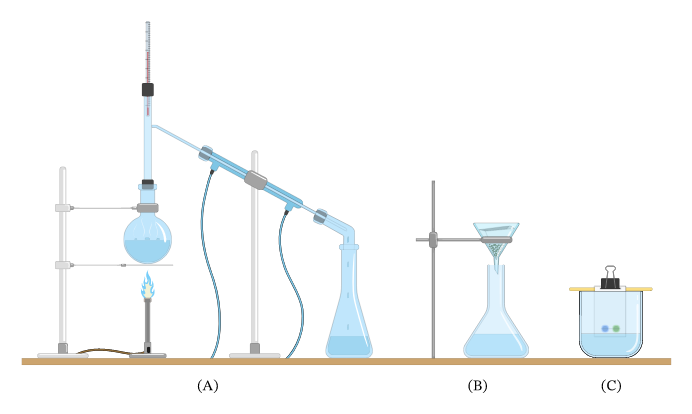
\includegraphics[scale=0.3]{../Listas/destilador.png}
\end{center}

\begin{choice}
\choice A: Destilação B: Filtração C: Cromatografia
\choice A: Peneiramento B: Filtração C: Cromatografia
\choice A: Destilação B: Evaporação C: Cromatografia
\choice A: Destilação Fracionada B: Evaporação C: Cromatografia
\choice A: Destilação B: Filtração C: Decantação
\end{choice}
\end{exercise}
\begin{solution}
Letra A
\end{solution}


\begin{exercise}
Qual é o nome da técnica de separação que está sendo executada no diagrama?


\begin{center}
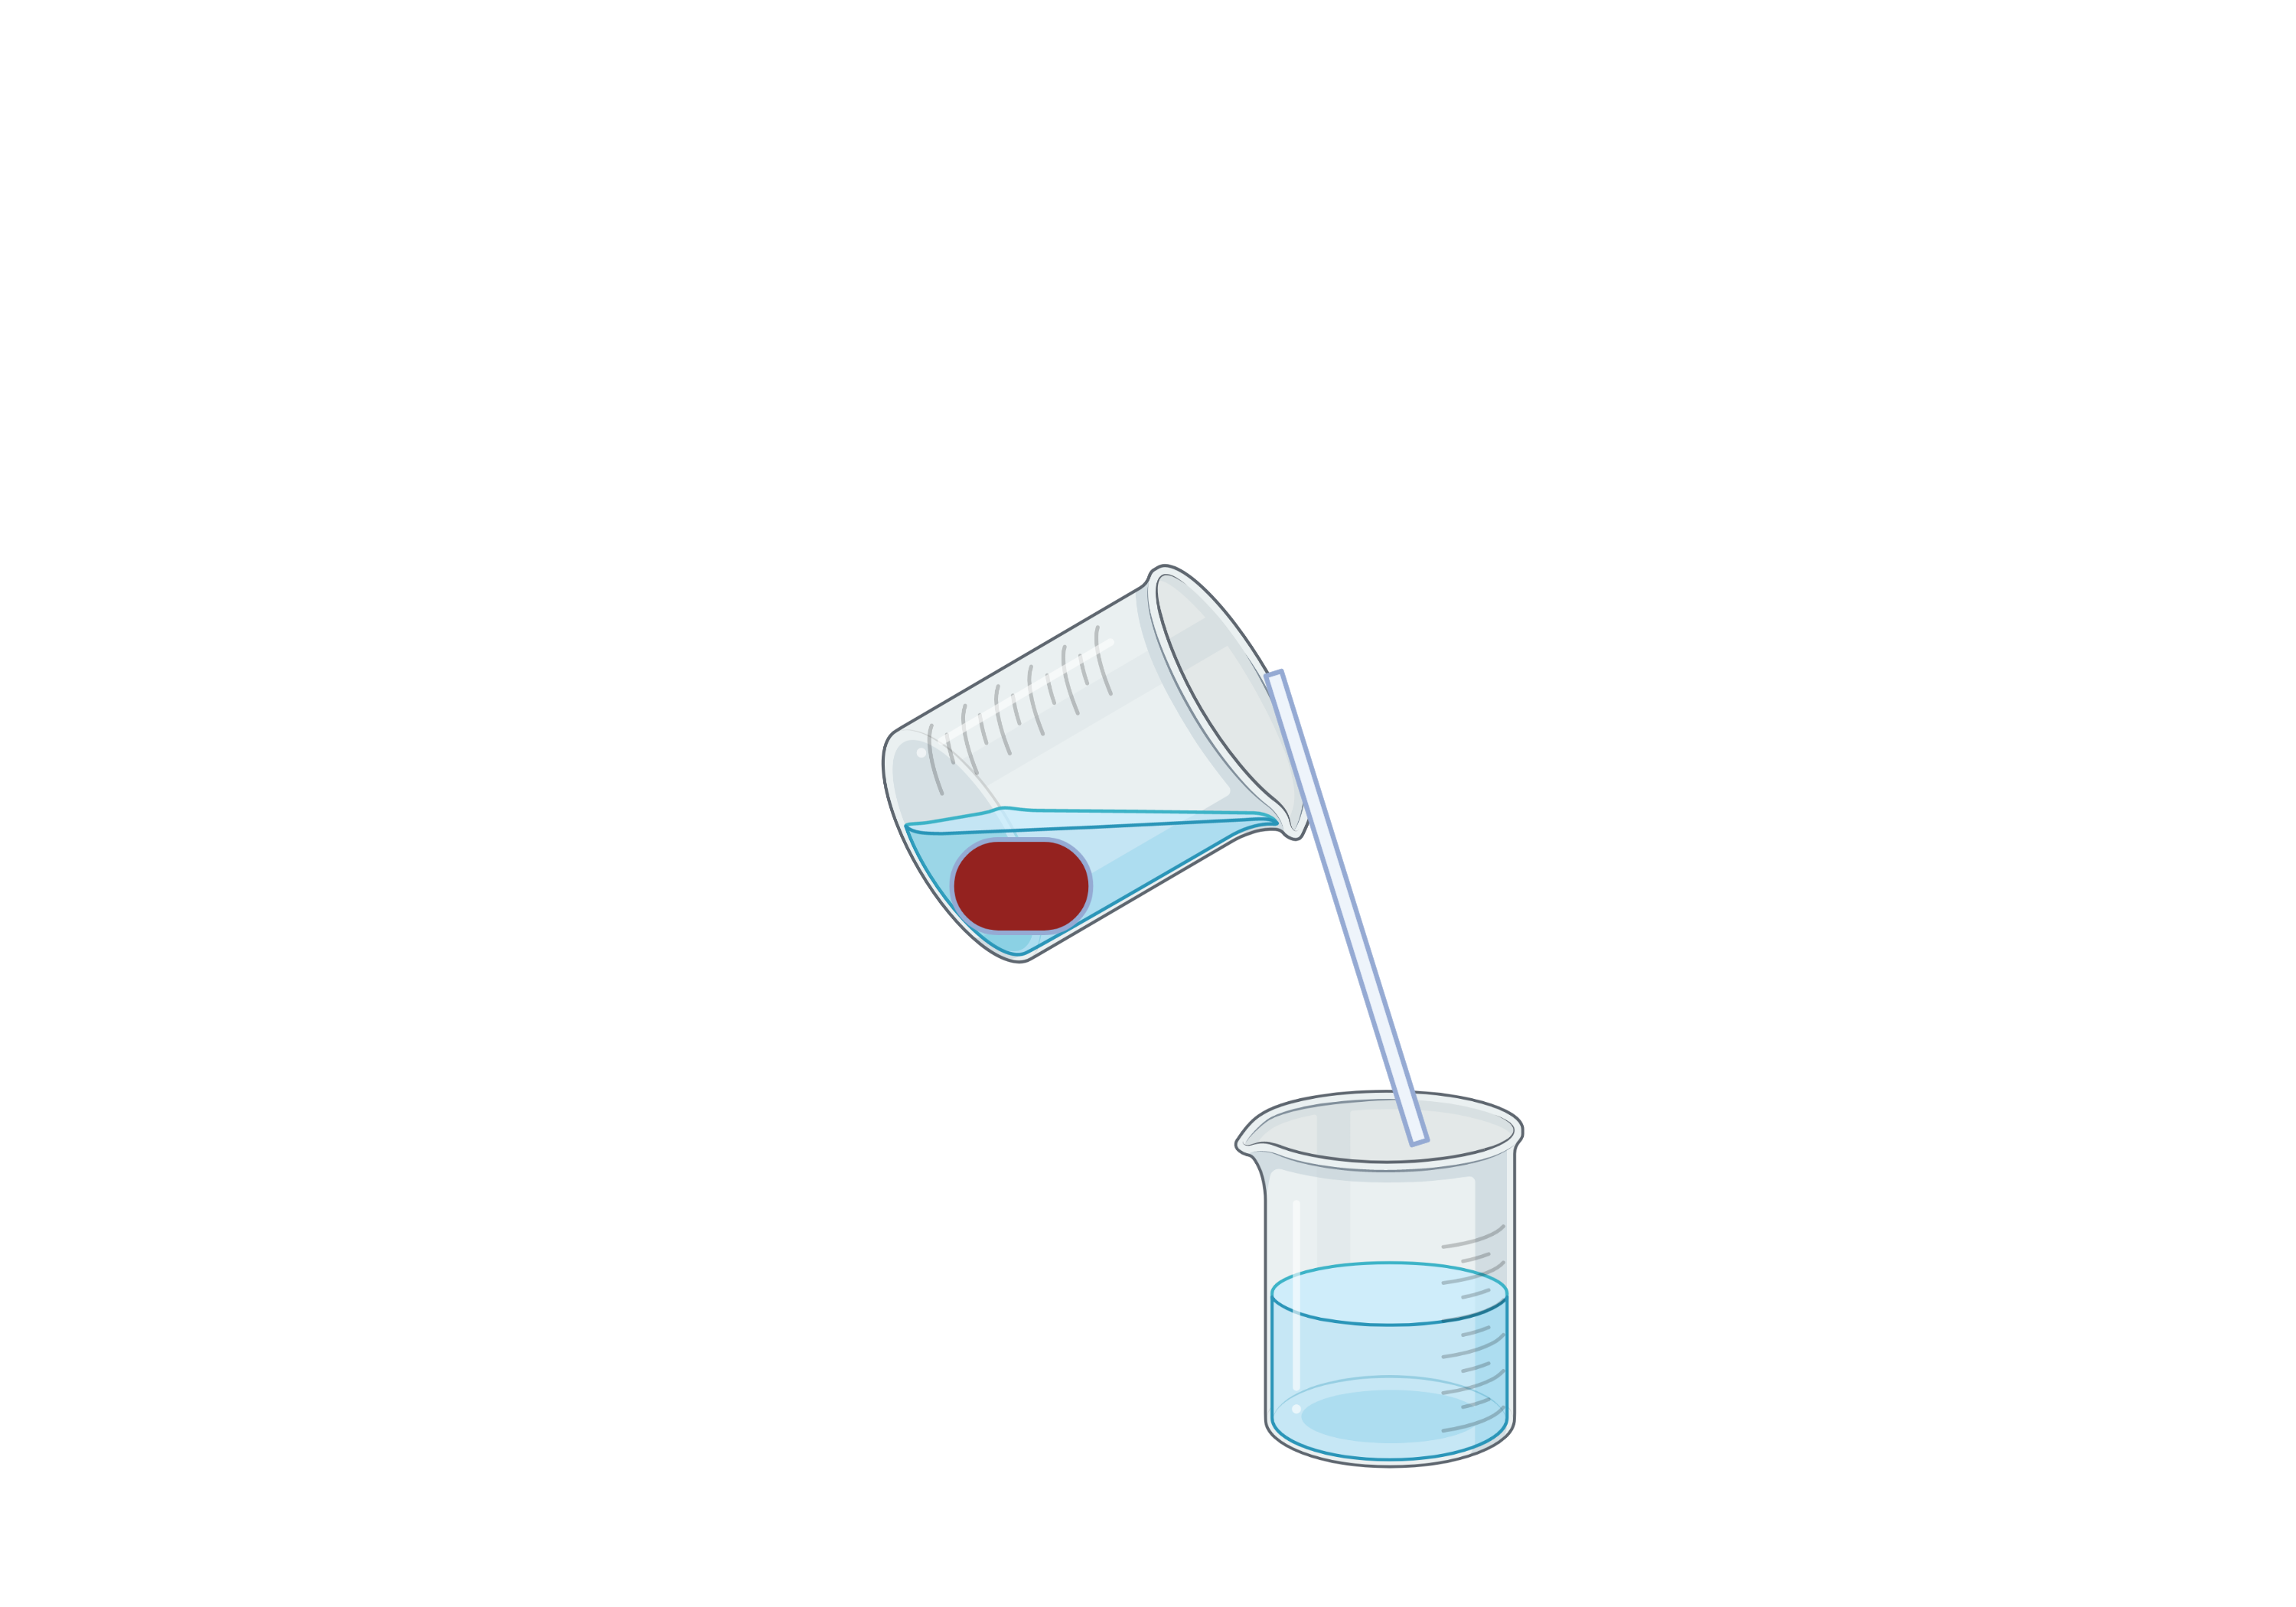
\includegraphics[scale=0.3]{../Listas/decanta.png}
\end{center}

\begin{choice}(2)
\choice Evaporação
\choice Filtragem
\choice Cromatografia
\choice Destilação
\choice Decantação
\end{choice}
\end{exercise}
\begin{solution}
Letra E
\end{solution}







\collectexercisesstop{ListaMisturas}






\collectexercises{LawProust}


\begin{exercise}
Uma das alternativas para diminuir a quantidade de dióxido de carbono liberada para a atmosfera consiste em borbulhar esse gás em solução aquosa de hidróxido de sódio. A reação que ocorre pode ser representada da seguinte forma:

\begin{reactions*}
\text{dióxido\; de\; carbono} + \text{hidróxido\; de\; sódio} -> &\\  \text{carbonato\; de\; sódio} + \text{água}
\end{reactions*}
Sabendo que 44 g de dióxido de carbono reagem com o hidróxido de sódio, formando 106 g de carbonato de sódio e 18 g de água, qual é a massa de hidróxido de sódio necessária para que o gás carbônico seja totalmente consumido?

\begin{choice}
\choice 62 g.
\choice 112 g.
\choice 20 g.
\choice 80 g.
\choice 106 g.
\end{choice}
\end{exercise}
\begin{solution}
Letra D
\end{solution}



\begin{exercise}
Foram analisadas três amostras (I, II e III) de óxidos de enxofre, procedentes de fontes
distintas, obtendo-se os seguintes resultados:


\begin{center}
\begin{tabular}{llll}
\hline
Amostra & m (g) enxofre & m (g) oxigenio & massa amostra (g)\\
\hline
I & 0,32 & 0,32 & 0,64\\
II & 0,08 & 0,08 & 0,16\\
III & 0,32 & 0,48 & 0,80\\
\hline
\end{tabular}
\end{center}

\begin{choice}
\choice apenas as amostras I e III são do mesmo óxido.
\choice as amostras I, II e III são de óxidos diferentes.
\choice apenas as amostras I e II são do mesmo óxido.
\choice apenas as amostras II e III são do mesmo óxido.
\choice as amostras I, II e III são do mesmo óxido.
\end{choice}
\end{exercise}
\begin{solution}
Letra C
\end{solution}


\begin{exercise}
Um químico deseja separar todos os componentes que constituem um sistema heterogêneo formado pela mistura de um álcool, de uma base, areia e de um óleo. Determine o processo de separação adequado em \textbf{X}, \textbf{Y} e \textbf{Z}, sabendo que a base é um granulado solúvel no álcool.

\begin{center}
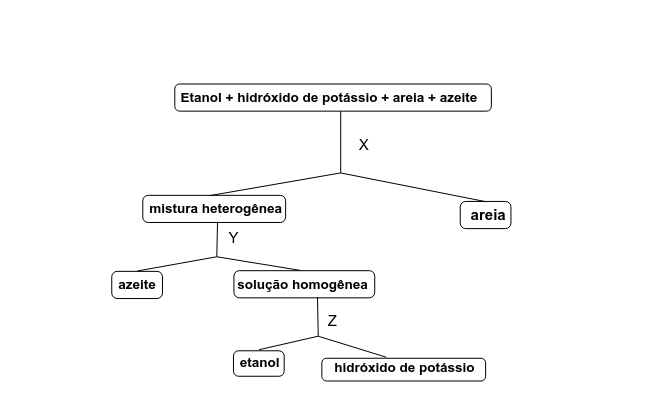
\includegraphics[scale=0.5]{../Listas/diagram-20230422.png}
\end{center}

Quais são o metódos usados em \textbf{x}, \textbf{y} e \textbf{z} ?


\blank[blank-style={\phantom{#1}},width=12\linewidth]{}
\end{exercise}




\begin{exercise}
Leia o texto.

“ -- Tudo que você vê faz parte de um delicado equilíbrio; como rei, você precisa entender esse equilíbrio a respeitar todas as criaturas, desde a formiguinha até o maior dos antílopes.
-- Mas, pais, nós não comemos os antílopes?
-- Sim, Simba, mas deixe-me explicar: quando morremos nossos corpos tornam-se grama e o antílope come a grama. E, assim, estamos todos conectados pelo grande ciclo da vida.”
{\small {\bfseries O REI LEÃO.} Walt Disney Productions, 1994.}

Considerando o texto

\begin{choice}
\choice explique como animais e vegetais incorporam e eliminam carbono;

\blank[blank-style={\phantom{#1}},width=12\linewidth]{}


\choice explique, à luz da lei de Lavoisier, por que “estamos todos conectados”.


\blank[blank-style={\phantom{#1}},width=12\linewidth]{}


\end{choice}
\end{exercise}




\collectexercisesstop{LawProust}






\collectexercises{ListaTeoriaAtomica}


\begin{exercise}
Quem introduziu pela primeira vez o princípio da incerteza?

\begin{choice}(2)
\choice Pauli
\choice De Broglie
\choice Dirac
\choice Schrödinger
\choice Heisenberg
\end{choice}
\end{exercise}
\begin{solution}
Letra E
\end{solution}




\begin{exercise}
Qual das alternativas a seguir \textbf{NÃO} é uma limitação do modelo de Bohr do átomo?

\begin{choice}
\choice Os elétrons se movem ao redor do núcleo em órbitas circulares e planas.
\choice Os elétrons são considerados apenas como partículas e não como ondas.
\choice É possível determinar com precisão a posição e o momento de um elétron simultaneamente.
\choice Os elétrons dentro dos átomos só podem ocupar níveis de energia quantizados.
\choice Ele explica apenas o espectro de emissão de linha do átomo de hidrogênio.
\end{choice}
\end{exercise}
\begin{solution}
C
\end{solution}




\begin{exercise}
Qual das seguintes afirmações é \textbf{verdadeira} sobre um elétron?

\begin{choice}
\choice Está localizado mais longe do núcleo quando absorve energia.
\choice Absorve energia quando se move de um estado de maior energia para o estado fundamental.
\choice Está localizado no núcleo quando absorve energia.
\choice Está localizado mais perto do núcleo quando absorve energia.
\choice Quando libera energia se move para um estado de maior energia
\end{choice}
\end{exercise}
\begin{solution}
E
\end{solution}




\begin{exercise}
Qual das alternativas a seguir melhor descreve um \textbf{elétron}?
\begin{choice}
\choice Uma partícula carregada positivamente com uma massa muito menor que a do núcleo
\choice Uma partícula carregada negativamente com uma massa muito menor que a do núcleo
\choice Uma partícula carregada positivamente com uma massa muito maior que a do núcleo
\choice Uma partícula carregada negativamente com uma massa muito maior que a do núcleo
\choice Partícula neutra com massa igual à do núcleo.
\end{choice}
\end{exercise}
\begin{solution}
D
\end{solution}




\begin{exercise}
Qual das alternativas a seguir melhor define o \textbf{número atômico} ?

\begin{choice}
\choice O número total de prótons e nêutrons no núcleo de um átomo
\choice O número de prótons no núcleo de um átomo
\choice O número de nêutrons no núcleo de um átomo
\choice O número total de prótons, nêutrons e elétrons em um átomo
\choice O número de elétrons no núcleo de um átomo
\end{choice}
\end{exercise}
\begin{solution}
A
\end{solution}






\begin{exercise}
Uma moda recente entre as crianças é colecionar figurinhas que brilham no escuro. As figuras apresentam em sua constituição, a substância sulfeto de zinco. O fenômeno ocorre porque alguns elétrons que compõem os átomos de zinco absorvem energia luminosa, saltando para níveis de energia mais externos. No escuro, esses elétrons retornam aos seus níveis de origem, liberando energia luminosa e fazendo a figurinha brilhar.

Essa característica pode ser explicada considerando o modelo atômico proposto por:

\begin{choice}
\choice Bohr.
\choice Rutherford.
\choice Lavoisier.
\choice Thomson.
\choice Dalton.
\end{choice}
\end{exercise}
\begin{solution}
A
\end{solution}




\begin{exercise}
Qual das imagens a seguir representa melhor o modelo atômico do pudim de passas de Thomson?


\begin{choice}
\choice \resizebox{.2\textwidth}{!}{%
\begin{circuitikz}
\tikzstyle{every node}=[font=\LARGE]
\draw  (2,12.25) circle (1.75cm);
\draw  (1,13.25) circle (0.25cm);
\draw  (2,13.25) circle (0.25cm);
\draw  (1.5,12) circle (0.25cm);
\draw  (2.75,12.25) circle (0.25cm);
\draw  (2.25,11.25) circle (0.25cm);
\node [font=\LARGE] at (1.5,11) {+};
\node [font=\LARGE] at (3,13) {+};
\node [font=\LARGE] at (2.5,11.5) {+};
\node [font=\LARGE] at (0.75,12.25) {+};
\node [font=\LARGE] at (2,12.5) {+};
\node [font=\LARGE] at (2.25,11.25) {-};
\node [font=\LARGE] at (2.75,12.25) {-};
\node [font=\LARGE] at (2,13.25) {-};
\node [font=\LARGE] at (1,13.25) {-};
\node [font=\LARGE] at (1.5,12) {-};
\end{circuitikz}
}%


\choice \resizebox{.2\textwidth}{!}{%
\begin{circuitikz}
\tikzstyle{every node}=[font=\LARGE]
\draw [fill={rgb, 255:red, 122; green, 119; blue, 119 }  ,fill opacity=1 ] (2,12.25) circle (1.75cm);
\end{circuitikz}
}%







\choice 	\resizebox{0.2\textwidth}{!}{%
		\begin{circuitikz}
			\tikzstyle{every node}=[font=\LARGE]
			\draw  (2,12.25) circle (1.75cm);
			\draw  (0.75,12.25) circle (0.25cm) node {\LARGE -} ;
			\draw  (1.5,13.25) circle (0.25cm);
			\draw  (3,12.5) circle (0.25cm);
			\draw  (2.25,11) circle (0.25cm) node {\LARGE -} ;
			\draw  (2,12.25) circle (0.5cm);
			\node [font=\huge] at (2,12.25) {+};
			\node [font=\large] at (1.5,13.25) {-};
			\node [font=\large] at (3,12.5) {-};
		\end{circuitikz}
	}%

\choice \resizebox{.2\textwidth}{!}{%
\begin{circuitikz}
\tikzstyle{every node}=[font=\LARGE]
\draw  (2,12.25) circle (1.75cm);
\draw [ fill={rgb,255:red,192; green,191; blue,188} ] (2,10.5) circle (0.25cm) node {\LARGE -} ;
\draw [ fill={rgb,255:red,192; green,191; blue,188} ] (0.25,12) circle (0.25cm) node {\LARGE -} ;
\draw [ fill={rgb,255:red,192; green,191; blue,188} ] (2,14) circle (0.25cm) node {\LARGE -} ;
\draw [ fill={rgb,255:red,192; green,191; blue,188} ] (3.75,12) circle (0.25cm) node {\LARGE -} ;
\draw  (2,12.25) circle (0.5cm) node {\LARGE +} ;
\end{circuitikz}
}%



\choice \resizebox{.2\textwidth}{!}{%
\begin{circuitikz}
\tikzstyle{every node}=[font=\LARGE]
\draw  (2,12.25) circle (1.75cm);
\draw  (2,12.25) circle (0.5cm) node {\LARGE +} ;
\end{circuitikz}
}%

\end{choice}
\end{exercise}





\begin{exercise}
Qual químico descobriu que os elétrons existem em níveis de energia fixos?
\#+begin\textsubscript{choice} 
\choice Bohr
\choice Thomson
\choice Dalton
\choice Geiger e Marsden
\choice Rutherford
\end{exercise}
\begin{solution}
A
\end{solution}



\begin{exercise}
Na experiência de Geiger-Marsden supervisionada por Ernest Rutherford (conhecida como a experiência da folha de ouro de Rutherford), que tipo de partícula foi dispersada por uma folha de ouro, provando que os átomos contêm um núcleo denso?

\begin{choice}
\choice Raios gama
\choice Nêutrons
\choice Partículas \(\Beta^+\)
\choice Partículas \(\Beta^-\)
\choice Partículas \(\alpha\)
\end{choice}
\end{exercise}

\begin{solution}
E
\end{solution}


\begin{exercise}
Qual é a principal força atrativa entre partículas no núcleo de um átomo?

\begin{choice}
\choice Gravidade
\choice Forca eletrostática
\choice Força nuclear forte
\choice Força nuclear fraca
\choice Força eletromagnética
\end{choice}
\end{exercise}
\begin{solution}
C
\end{solution}


\begin{exercise}
Que passo em frente, a partir do modelo atômico das orbitais de Bohr, foi dado por Schrödinger no seu modelo da nuvem eletrónica?

\begin{choice}
\choice O núcleo contém partículas com massa mas sem carga.
\choice Os elétrons ocupam níveis de energia com raios fixos.
\choice O núcleo contém partículas com massa e carga positiva.
\choice Os elétrons movem-se dentro de uma esfera positivamente carregada.
\choice Os elétrons estão dispersos no espaço.
\end{choice}
\end{exercise}
\begin{solution}
E
\end{solution}



\begin{exercise}
Em que é que o modelo atômico de Thomson é diferentes do modelo atômico de Dalton?

\begin{choice}
\choice O modelo atômico de Thomson inclui partículas com carga negativa conhecidas como elétrons
\choice O modelo atômico de Thomson mostra elétrons a ocupar os vértices de um cubo.
\choice O modelo atômico de Thomson inclui partículas com carga positiva conhecidas como prótons
\choice O modelo atômico de Thomson descreve elétrons a orbitar um núcleo central.
\choice O modelo atômico de Thomson mostra elétrons a ocupar diferentes níveis de energia.
\end{choice}
\end{exercise}
\begin{solution}
A
\end{solution}




\collectexercisesstop{ListaTeoriaAtomica}







\collectexercises{ListaBalanceamento}

\begin{exercise}
Balanceie as reações químicas:
\begin{choice}(1)
\choice \ch{\lh Fe + \lh C$\ell$2 -> \lh FeC$\ell$3} \bigskip \bigskip
\choice \ch{\lh Fe + \lh O2 -> \lh Fe2O3} \bigskip \bigskip
\choice \ch{\lh FeBr3 + \lh H2SO4 -> \lh Fe2(SO4)3 + \lh HBr}\bigskip \bigskip
\choice \ch{\lh C4H6O3 + \lh H2O  ->  \lh C2H4O2} \bigskip \bigskip
\choice \ch{\lh C2H4 + \lh O2 -> \lh CO2 + \lh H2O} \bigskip \bigskip
%\choice \ch{\lh C4H10O + \lh O2 -> \lh CO2 + \lh H2O} \bigskip \bigskip
\choice \ch{\lh C7H16 + \lh O2 -> \lh  CO2 + \lh  H2O} \bigskip \bigskip
%\choice \ch{\lh H2SiC$\ell$2 + \lh H2O -> \lh H8Si4O4 + \lh HC$\ell$} \bigskip \bigskip
%\choice \ch{\lh HSiC$\ell$3 + \lh H2O -> \lh H10Si10O15 + \lh HC$\ell$} \bigskip \bigskip
\choice \ch{\lh C7H9 + \lh HNO3 -> \lh C7H6(NO2)3 + \lh H2O} \bigskip \bigskip
%\choice \ch{\lh C5H8O2 + \lh NaH + \lh HCl -> \lh C5H12O2 + \lh NaC$\ell$} \bigskip \bigskip
\choice \ch{\lh Fe + \lh H2SO4 \ -> \lh Fe2(SO4)3 + \lh H2} \bigskip \bigskip
\choice \ch{\lh C2H6 + \lh O2 -> \lh H2O + \lh CO2} \bigskip  \bigskip
\choice \ch{\lh KOH + \lh H3PO4 -> \lh K3PO4 + \lh H2O} \bigskip \bigskip
\choice \ch{\lh SnO2 + \lh H2 -> \lh Sn + \lh H2O} \bigskip \bigskip
\choice \ch{\lh NH3 + \lh O2 -> \lh NO  + \lh  H2O} \bigskip \bigskip
\choice \ch{\lh KNO3 + \lh H2CO3 -> \lh K2CO3 + \lh HNO3} \bigskip \bigskip 
\choice \ch{\lh B2Br6 + \lh HNO3 -> \lh  B(NO3)3 + \lh HBr} \bigskip \bigskip
\choice \ch{\lh BF3 + \lh  Li2SO3 -> \lh B2(SO3)3 + \lh LiF} \bigskip \bigskip
\choice \ch{\lh (NH4)3PO4 + \lh  Pb(NO3)4  -> \lh Pb3(PO4)4  + \lh NH4NO3} \bigskip \bigskip
%%\choice \ch{\lh SeC$\ell$6  + \lh  O2 -> \lh  SeO2 + \lh C$\ell$2} \bigskip \bigskip
\choice \ch{\lh HC$\ell$O4 + \lh P4O10  -> \lh H3PO4 + \lh C$\ell$2O7} \bigskip \bigskip
\choice \ch{\lh Ca3(PO4)2  + \lh H2SO4 -> \lh CaSO4  + \lh Ca(H2PO4)2} \bigskip \bigskip
%%\choice \ch{\lh FeO3  + \lh CO -> \lh Fe  + \lh CO2} \bigskip \bigskip
\choice \ch{\lh CO + \lh H2 -> \lh  C8H18 + \lh H2O}
\end{choice}
\end{exercise}



\collectexercisesstop{ListaBalanceamento}
\end{document}
